\graphicspath{{./ThirdTask/}} % path to graphics

\section*{\LARGE Цель практической работы}
\addcontentsline{toc}{section}{Цель практической работы}

\textbf{Цель работы:} изучить основные элементы и правила построения, а также
сформировать навык построения диаграммы последовательности в Visual
Paradigm.

\textbf{Задачи:}\par
\begin{itemize}
	\item познакомиться с назначением диаграммы последовательности, ее
		элементами, правилами и этапами построения;
	\item построить диаграмму последовательности в Visual Paradigm в
		соответствии с предложенными заданиями.
\end{itemize}

\newpage

\section*{\LARGE Выполнение практической работы}
\addcontentsline{toc}{section}{Выполнение практической работы}
\section{Краткая теория}
Диаграмма последовательности описывает взаимодействие элементов
какой-либо системы (например, ERP-системы) во времени, и организованы в
соответствии с объектами по горизонтали и временем по вертикале. Как
правило объекты размещаются слева0 направо в зависимости от того, в какой
последовательности они вступают во взаимодействие. Время указывается в
порядке последовательности и не отражает аспект длительности.\par
Диаграмма последовательности отражает динамический аспект
взаимодействия элементов системы.\par
На диаграмме последовательности изображаются объекты, которые
непосредственно участвуют во взаимодействии, при этом никакие статические
связи с другими объектами не визуализируются. Для диаграммы
последовательности ключевым моментом является именно динамика
взаимодействия объектов во времени. При этом можно сказать, что диаграмма
последовательности имеет два измерения. Одно - слева направо в виде
вертикальных линий, каждая из которых изображает линию жизни отдельного
объекта, участвующего во взаимодействии. Графически каждый объект
изображается прямоугольником и располагается в верхней части своей линии
жизни.\par
На уровне реализации с помощью диаграммы последовательности моделируется
взаимодействие между отдельными компонентами информационной системы.

\section{Построение диаграммы последовательности}
Клиентом на данной диаграмме изображен актер по имени "<Клиент">.
Для помещения на диаграмму "<Клиент"> достаточно перетащить
соответствующий элемент Actor.
Вначале он авторизуется на сайте вводя свой логин и парол, для этого
вводится объект "<Личный кабинет пользователя">.
Для представления "<Личного кабинета пользователя"> Интернет-магазина
достаточно перенести на диаграмму элемент LifeLine и переименовать ее
соответствующим образом.
Для отражения запроса клиента необходимо выбрать
стрелку Send message из выпадающего меню с сообщениями.
Аналогичным способом строится остальная диаграмма.\par
Для условной логики можно использовать оператор alt и помещать
условие в каждый фрагмент.Итоговая диаграмма проиллюстрированна на рисурнке~\ref{fig:sequence}.

\begin{figure}[h!tp]
	\centering
	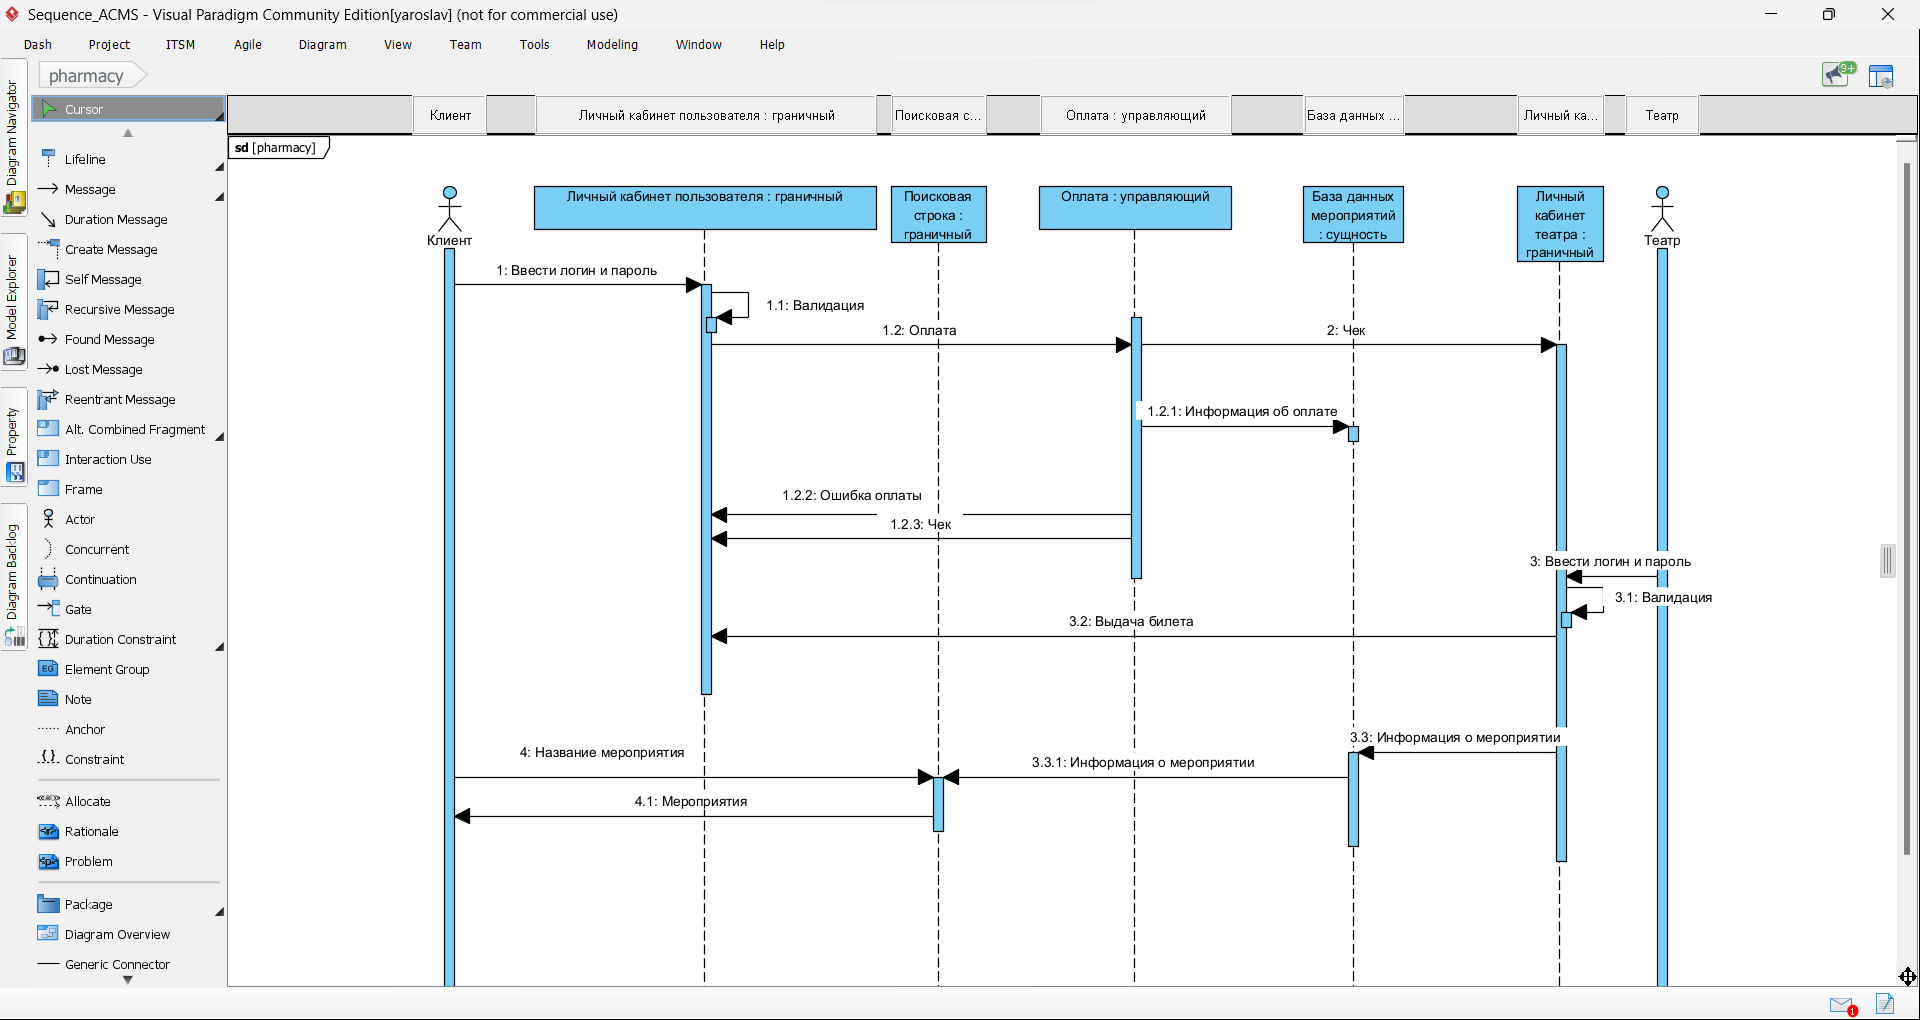
\includegraphics[width=1\textwidth]{img.png}
	\caption{Диаграмма последовательности}
	\label{fig:sequence}
\end{figure}

\newpage

\section*{Ответы на вопросы}
\addcontentsline{toc}{section}{Ответы на вопросы}

\begin{description}
	\item[Дайте определение понятию «диаграмма последовательности» и опишите
		ее назначение. Приведи примеры ситуаций, когда целесообразно ее
		использовать.]
		\textit{Диаграмма последовательности} описывает взаимодействие
		элементов какой-либо системы (например, ERP-системы) во времени,
		и организованы в соответствии с объектами по горизонтали и временем
		по вертикале.
	\item[Какова роль диаграмм развертывания в проектировании информационных
		систем?]
		\textit{Диаграмма развертывания} предназначена для
		представления общей конфигурации или топологии распределения
		программной системы и содержит изображение размещения различных
		артефактов по отдельным узлам системы.
	\item[В каких случаях целесообразно использовать оператор
		взаимодействия alt?]
		Для описания условной логики. Тогда условие помещается в каждый
		фрагмент и будет выполнен только тот фрагмент, значение
		которого имеет истинное значение.
	\item[Охарактеризуйте линию жизни объекта и представьте ее графическое
		изображение.]
		\textit{Линия жизни} служит для обозначения периода времени, в
		течение которого объект существует в системе и может
		потенциально участвовать во всех ее взаимодействиях. Если
		объект существует в системе постоянно, то его пунктирная
		линия должна продолжаться по всей рабочей области
		диаграммы последовательности от самой верхней ее части до
		самой нижней (Рисунок~\ref{fig:lineLive}).
		\begin{figure}[h!tp]
			\centering
			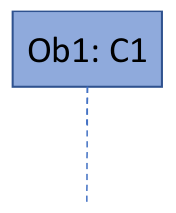
\includegraphics[width=0.2\textwidth]{Screenshot from 2023-03-18 18-02-21.png}
			\caption{Обозначение линии жизни}
			\label{fig:lineLive}
		\end{figure}
	\item[Для чего предназначен фокус управления? Представьте его графическое
		изображение.]
		\textit{Фокус управления} --- специальный
		символ на диаграмме последовательности,
		указывающий период времени, в течение которого
		объект выполняет некоторое действие, находясь в
		активном состоянии (Рисунок~\ref{fig:mngfck}).
		\begin{figure}[h!tp]
			\centering
			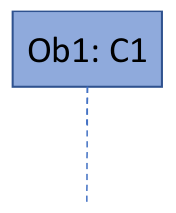
\includegraphics[width=0.2\textwidth]{Screenshot from 2023-03-18 18-02-21.png}
			\caption{Обозначение линии жизни}
			\label{fig:mngfck}
		\end{figure}
	\item[Сформулировать определение понятия «сообщение». Какие виды
		сообщений используются в диаграмме последовательности?]
		\textit{Сообщения} --- это законченный фрагмент
		информации, который отправляется одним объектом
		другому. Прием сообщения инициирует выполнение
		определенных действий, направленных на решение
		отдельной задачи тем объектом, которому это
		сообщение отправлено.
		Используются:
		\begin{itemize}
			\item синхронные;
			\item асинхронные;
			\item ответное или возврат;
			\item найденное;
			\item потерянное;
			\item рекурсивный вызов.
		\end{itemize}
	\item[Когда используется рефлексивное сообщение?]
		Когда участник отправляет сообщение (команду) самому себе.
	\item[Расскажите про ветвления на диаграмме последовательности. Приведите
		пример ветвления.]
		Наиболее простые случаи ветвления процесса взаимодействия можно
		изобразить на одной диаграмме с использованием соответствующих
		графических операторов или операндов (Рисунок~\ref{fig:apt}).
		\begin{figure}[h!tp]
			\centering
			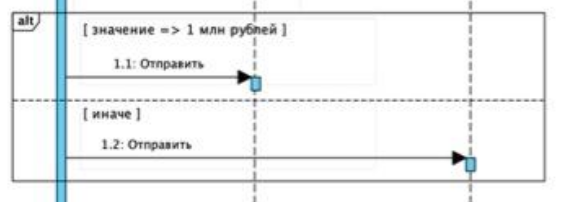
\includegraphics[width=0.8\textwidth]{Screenshot from 2023-03-18 18-14-47.png}
			\caption{Пример ветвления}
			\label{fig:apt}
		\end{figure}
	\item[В каких случаях целесообразно использовать оператор
		взаимодействия opt?]
		Для обозначения случая, когда один операнд либо выполняется, либо нет.
	\item[Охарактеризуйте понятие оператора взаимодействия.]
		Оператор определяет операцию о том, как будут выполняться операнды.
	\item[В каких случаях целесообразно использовать
		операторы взаимодействия?]
		Для обозначения не тривиальных случаев взаимодействия между
		объектами или актерами.
\end{description}

\newpage

\section*{\LARGE Вывод}
\addcontentsline{toc}{section}{Вывод}
В результате практическои работы ознакомились с назначением диаграммы
последовательности, ее элементами, правилами и этапами построения.
Получили предоставление о программе Visual Paradigm, предназначенной
для построения диаграммы последовательности.
А также научились строить диаграмму последовательности в Visual Paradigm в
соответствии с предложенным вариантом.
